\documentclass{beamer}
\usetheme{Boadilla}

\usepackage{amsmath}
\usepackage{amsfonts}
\usepackage{hyperref}
\usepackage{amsthm}



\title{f-Divergence Variational Inference}
\author{Skorik Sergey}
\institute{MIPT, 2022}


\begin{document}

\begin{frame}
    \titlepage
\end{frame}


\begin{frame}
    \tableofcontents
\end{frame}

\section{Preliminaries}

\begin{frame}{Motivation}
    \begin{block}{Introduction}
        Let consider the \textbf{Bayesian inference}
        $$p(z|x) = \dfrac{p(z,x)}{p(x)}$$
        MCMC algorithms estimate the evidence $p(x) = \int p(z, x) dx$ via sampling. However, since sampling tends to be a slow and computationally intensive process, VI becomes a good alternative to perform Bayesian inference. Let's denote a family of approximate densities $\mathcal{Q}$. The VI problem is to find the member $q^*(z) \in \mathcal{Q}$ that minimizes the distance between the true posterior $D(q(z) || p(z|x))$. This distance called \textbf{divergence}. 

        Some examples of divergences:
        \begin{enumerate}
            \item Kullback-Leibler: $\int p(x) \frac{p(x)}{q(x)}dx$
            \item Pearson $\chi^2$: $\int \frac{(q(x) - p(x))^2}{p(x)}dx$
        \end{enumerate}
    \end{block}
\end{frame}

\begin{frame}{f-divergence}
    \begin{block}{}
        \textbf{Definition 1} \textit{The f-divergence from probability density functions $q(z)$ to $p(z)$ is defined as}
        \begin{equation}\label{def1}
            D_f(q(z)||p(z)) =: \int f\left(\dfrac{q(z)}{p(z)}\right)p(z) dz = \mathbb{E}_p\left[f\left(\dfrac{q(z)}{p(z)}\right)\right],
        \end{equation}
        where $f(\cdot)$ is a convex function with $f(1)=0$.

        \begin{table}[]
        \caption{Divergences $D_f(q||p)$}
        \begin{tabular}{|l|l|}
        \hline
        Divergences                                        & $f(t)$                              \\ \hline
        KL divergecne                                      & $t\log t$                           \\ \hline
        General $\chi^n$-divergence                           & $t^n - 1$, $n\in \mathbb{R}\symbol{92}(0, 1)$ \\ \hline
        Hellinger $\alpha$-divergence $\mathcal{H_\alpha}$ &   $(t^\alpha - 1) \slash (\alpha - 1)$, $\alpha\in\mathbb{R}^+\symbol{92}\{1\}$                                  \\ \hline
        \end{tabular}
        \end{table}
    \end{block}
\end{frame}

\begin{frame}{f-divergence}
    \begin{block}{}
        \textbf{Definition 2} \textit{Given a function $f: (0,1) \rightarrow \mathbb{R}$, the dual function $f^*: (0,1)\rightarrow \mathbb{R}$ is defined as}
        \begin{equation*}
            f^*(t) = t \cdot f(1\slash t)
        \end{equation*}
        \textbf{Properties:}
        \begin{enumerate}
            \item $(f^*)^* = f$
            \item if $f$ is convex, $f^*$ is also convex
            \item if $f(1)=0$, then $f^*(1)=0$
            \item With dual function $f^*$ an identity between the forward and reverse $f$-divergences can be established 
            $$D_{f^*}(p||q) = \int \dfrac{p(z)}{q(z)}f\left(\dfrac{q(z)}{p(z)}\right)q(z) dz = D_f(q||p)$$
        \end{enumerate}
    \end{block}
\end{frame}

\begin{frame}{f-divergence}
    \begin{block}{}
        In order to facilitate the derivation of f-variational bound, especially when the latent variable model is involved, we introduce a \textit{surrogate f-divergence} $D_{f_\lambda}$ defined by the \textit{generator function}
        \begin{equation}\label{f_lambda}
            f_\lambda(\cdot) = f(\lambda\cdot) - f(\lambda)
        \end{equation}
        where $\lambda \geqslant 0$ is a constant. 
    \end{block}
    \begin{block}{Proposition}
        \textbf{Proposition 1:} Given two probability distributions $q$ and $p$, a convergent sequence $\lim_{n\to\infty}\lambda_n = 1$, $\lambda_n \geqslant 0$ and a convex function $f: (0, +\infty) \rightarrow \mathbb{R}$ such that $f(1)=0$ and $f(\cdot)$ is uniformly continuous, the $f$-divergences between $q$ and $p$ satisfy
        \begin{equation}\label{prop1}
            D_{f_{\lambda_n}}(q||p) \rightarrow D_f(q||p)
        \end{equation}
        almost everywhere as $n\to\infty$
    \end{block}
\end{frame}

\begin{frame}{f-divergence}
    \begin{block}{Proof}
        \textbf{Proof:}

        $$\lim\limits_{n\to\infty}D_{f_{\lambda_n}}(q||p) = \lim\limits_{n\to\infty}\int p(z) \left[f\left(\lambda_n\dfrac{q(z)}{p(z)}\right) - f(\lambda_n)\right] dz =$$
        $$= \lim\limits_{n\to\infty}\int p(z) f\left(\lambda_n\dfrac{q(z)}{p(z)}\right)dz - \lim\limits_{n\to\infty}f(\lambda_n) \int p(z)dz =$$
        $$= \int \lim\limits_{n\to\infty} p(z) f\left(\lambda_n\dfrac{q(z)}{p(z)}\right)dz = D_f(q||p)$$
    \end{block}
\end{frame}

\begin{frame}{Shifted homogeneity}
    \begin{block}{}
        We then introduce a class of $f$-functions equipped with a structural advantage in decomposition, which will be invoked later to derive the coordinate-wise VI algorithm under mean-field assumption.

        \textbf{Definition 3} A convex function $f$ belongs to $\mathcal{F}_{\{0, 1\}}$, if $f(1)=0$ and for any $t, \Tilde{t} \in \mathbb{R}$ we have
        \begin{equation}\label{def3}
            f(t\Tilde{t}) = t^\gamma f(\Tilde{t}) + f(t)\Tilde{t}^\eta,
        \end{equation}
        where $\gamma\in\mathbb{R}$ and $\eta\in\{0, 1\}$. Function $f$ is type $0$ shifted homogeneous or $f \in \mathcal{F}_0$ if $\eta = 0$, and type 1 shifted homogeneous or $f \in \mathcal{F}_1$ if $\eta = 1$.
    \end{block}
\end{frame}

\begin{frame}{Shifted homogeneity}
    \begin{block}{Propositions}
        The duality property between F0 and F1 is stated in Proposition 2.

        \textbf{Proposition 2} Given $f_0 \in \mathcal{F}_0$ and $f_1 \in \mathcal{F}_1$, the dual functions $f_0^* \in \mathcal{F}_1$ and $f_1^* \in \mathcal{F}_0$. 

        When $f \in \mathcal{F}_{\{0,1\}}$, we can establish a more profound relationship, in contrast with Proposition 1, between $f$-divergence $D_f$ and surrogate divergence $D_{f_\lambda}$

        \textbf{Proposition 3} When $f \in \mathcal{F}_{\{0,1\}}$ and $\lambda > 0$ , an $f$-divergence $D_f$ and its surrogate divergence $D_{f_\lambda}$ satisfy
        \begin{equation}\label{prop3}
            D_{f_{\lambda}}(q||p) = \lambda^\gamma D_f(q||p)
        \end{equation}
    \end{block}
\end{frame}

\begin{frame}{Shifted homogeneity}
    \begin{block}{Proofs}
        \textbf{Proof of Proposition 2}. Let $f_0 \in \mathcal{F}_0$. Since
        $$f^*(t\Tilde{t}) = t\Tilde{t}\cdot f\left(\dfrac{1}{t\Tilde{t}}\right) = t\Tilde{t}\left[\left(\dfrac{1}{t}\right)^{\gamma_0}\cdot f\left(\dfrac{1}{\Tilde{t}}\right) + f\left(\dfrac{1}{t}\right)\right]=$$
        $$= t^{1-\gamma_0}\cdot f^*_0(\Tilde{t}) + f^*_0(t)\cdot\Tilde{t}$$
        by letting $\gamma=1-\gamma_0$  we can conclude that $f_0^*\in\mathcal{F}_1$. Case $f_1 \in \mathcal{F}_1$ proved analogous.

        \textbf{Proof of Proposition 3}. We start this proof by substituting \eqref{def1}, \eqref{f_lambda} and \eqref{def3} into the LHS of \eqref{prop3}
        $$D_{f_{\lambda}}(q||p) = \mathbb{E}_p[f_\lambda(q/p)] = \mathbb{E}_p[f(\lambda q/p)] - f(\lambda) = $$
        $$= \lambda^\gamma\mathbb{E}_p[f(q/p)] + f(\lambda)\mathbb{E}_p[(q/p)^\eta] - f(\lambda) = \lambda^\gamma D_f(q||p)$$
    \end{block}
\end{frame}

\section{f-variational bounds}

\begin{frame}{f-variational bounds}
    \begin{block}{}
        Given a convex function $f$ such that $f(1) = 0$ and a set of i.i.d. samples $\mathcal{D}=\{x^{(n)}\}_{n=1}^N$, the generator function $f_{p(\mathcal{D})^{-1}}$ with $p(\mathcal{D}) > 0$ can induce a surrogate f-divergence.
        \begin{equation}\label{surrograte_f_div}
            D_{f_{p(\mathcal{D})^{-1}}}(q(z)||p(z|\mathcal{D})) = \dfrac{1}{p(\mathcal{D})}\mathbb{E}_{q(z)}\left[f^*\left(\dfrac{p(z, \mathcal{D})}{q(z)}\right)\right] - f\left(\dfrac{1}{p(\mathcal{D})}\right)
        \end{equation}
        Multiplying both sides of \eqref{surrograte_f_div} by $p(\mathcal{D})$ and with rearrangements, we have
        \begin{equation}\label{L_f}
            \mathcal{L}_f(q, \mathcal{D}) = \mathbb{E}_{q(z)}\left[f^*\left(\dfrac{p(z, \mathcal{D})}{q(z)}\right)\right] = f^*(p(\mathcal{D})) + p(\mathcal{D})\cdot D_{f_{p(\mathcal{D})^{-1}}}(q(z)||p(z|\mathcal{D}))
        \end{equation}
    \end{block}
\end{frame}

\begin{frame}{f-variational bounds}
    \begin{block}{}
        \textbf{Theorem 1} Dual function of evidence $f^*(p(\mathcal{D}))$  is bounded above by f-variational bound $\mathcal{L}_f(q, \mathcal{D})$
        \begin{equation}\label{theo1}
            \mathcal{L}_f(q, \mathcal{D}) = \mathbb{E}_{q(z)}\left[f^*\left(\dfrac{p(z, \mathcal{D})}{q(z)}\right)\right] \geqslant f^*(p(\mathcal{D})),
        \end{equation}

        \textbf{Examples:}
        \begin{enumerate}
            \item KL-divergence: $f(t) = t\log t \Rightarrow f^*(t) = -\log t$ which is convex and decreasing. 
            $$\log p(\mathcal{D}) \geqslant \mathbb{E}_{q(z)}[\log p(z, \mathcal{D})] - \mathbb{E}_{q(z)}[\log q(z)] = ELBO$$
            \item $\chi^2$-divergence. $f(t) = t^{-1} - t \Rightarrow f^*(t) = t^2 - 1$, so
            $$\mathbb{E}_{q(z)}\left[\left(\dfrac{p(z, \mathcal{D})}{q(z)}\right)^2 - 1\right] \geqslant p(x)^2 - 1$$
            
        \end{enumerate}
    \end{block}
\end{frame}

\begin{frame}{Importance-weighted VI}
    \begin{block}{}
        \textbf{Corollary 1} When $1 \leqslant L_1 \leqslant L_2$, the importance-weighted f-variational bound $\mathcal{L}_f^{IW}(q, \mathcal{D}, L)$ and the f-variational bound $\mathcal{L}_f(q, \mathcal{D})$ satisfy
        $$\mathcal{L}_f(q, \mathcal{D}) \geqslant \mathcal{L}_f^{IW}(q, \mathcal{D}, L_1) \geqslant \mathcal{L}_f^{IW}(q, \mathcal{D}, L_2) \overset{L\to\infty}{\longrightarrow} f^*(p(\mathcal{D}))$$
        where $\mathcal{L}_f^{IW}(q, \mathcal{D}, L)$ is defined as
        $$\mathcal{L}_f^{IW}(q, \mathcal{D}, L) = \mathbb{E}_{z_{1:L}\sim q(z)}\left[f^*\left(\dfrac{1}{L}\sum_{l=1}^L\dfrac{p(z_l, \mathcal{D})}{q(z_l)}\right)\right]$$,
        and $z_{1:L} = \{z_l\}_{l=1}^L$ are $L \in \mathbb{N}$  i.i.d. samples from $q(z)$.
    \end{block}
\end{frame}

\begin{frame}{Sandwich formula}
    \begin{block}{}
        After composing both sides of \eqref{theo1} with the inverse dual function $(f^*)^{-1}$, we have the following observations:
        \begin{enumerate}
            \item When the dual function $f^*$ is increasing (or non-decreasing) on $\mathbb{R}^+$, the composition gives an evidence upper bound:
            $$(f^*)^{-1} \circ \mathcal{L}_f(q, \mathcal{D}) \geqslant p(\mathcal{D})$$
            \item When the dual function $f^*$ is decreasing (or non-increasing) on $\mathbb{R}^+$, the composition gives an evidence lower bound:
            $$(f^*)^{-1} \circ \mathcal{L}_f(q, \mathcal{D}) \leqslant p(\mathcal{D})$$
            \item When the dual function $f^*$ is non-monotonic on $\mathbb{R}^+$, the composition gives a local evidence bound by applying previous two observations on a monotonic interval $f^*$:
            $$(f^*)^{-1} \circ \mathcal{L}_f(q, \mathcal{D}) \geqslant p(\mathcal{D})$$
        \end{enumerate}
    \end{block}
\end{frame}

\begin{frame}{Sandwich formula}
    \begin{block}{}
        Based on these observations, we can readily imply a sandwich formula for evidence $p(\mathcal{D})$, which is essential for accurate VI.

        \textbf{Corollary 2} Given convex functions $f$ and $g$ such that $f(1) = g(1) = 0$ on an interval where $f^*$ is increasing and $g^*$ is decreasing the evidence $p(\mathcal{D})$ satisfy
        \begin{equation}\label{corol2}
            (g^*)^{-1} \circ \mathbb{E}_{q(z)}\left[g^*\left(\dfrac{p(z, \mathcal{D})}{q(z)}\right)\right] \leqslant p(\mathcal{D}) \leqslant (f^*)^{-1} \circ \mathbb{E}_{q(z)}\left[f^*\left(\dfrac{p(z, \mathcal{D})}{q(z)}\right)\right].
        \end{equation}
    \end{block}
\end{frame}

\section{Stochastic optimization}

\begin{frame}{Stochastic optimization}
    \begin{block}{}
        An intuitive approach to apply stochastic optimization is to compute the standard gradient of $\mathcal{L}_f(q, \mathcal{D})$ or $\mathcal{L}_f^{IW}(q, \mathcal{D})$ w.r.t. $\theta$
        \begin{equation}\label{L_f_grad}
            \nabla_{\theta}\mathcal{L}_f(q_\theta, \mathcal{D}) = \mathbb{E}_{q_\theta(z)}\left[f^{'}\left(\dfrac{q_\theta(z)}{p(z, \mathcal{D})}\right)\cdot\nabla_\theta\log q_\theta(z)\right],
        \end{equation}
        where $f^{'}(t)$ denotes $\partial f(t) \slash \partial t$.

        An unbiased Monte Carlo (MC) estimator for \eqref{L_f_grad} can be obtained by drawing $z_1, z_2, \ldots, z_K$ from $q_\theta(z)$ and
        \begin{equation}\label{L_f_estim}
            \nabla_{\theta}\hat{\mathcal{L}}_f(q_\theta, \mathcal{D}) = \dfrac{1}{K}\sum_{k=1}^K\left[f^{'}\left(\dfrac{q_\theta(z_k)}{p(z_k, \mathcal{D})}\right)\cdot\nabla_\theta\log q_\theta(z_k)\right]
        \end{equation}
    \end{block}
\end{frame}

\begin{frame}{Stochastic optimization}
    \begin{block}{}
        An alternative to the score function gradient is the reparameterization gradient, which empirically has a lower estimation variance. Let $\varepsilon \sim \mathcal{N}(0, 1)$ and $z = g_\theta(\varepsilon) = \mu + \Sigma^{\frac{1}{2}}\varepsilon$.
        
        The gradient of $\mathcal{L}_f(q, \mathcal{D})$ after reparameterization becomes
        \begin{equation}\label{L_f_repar}
            \nabla_{\theta}\mathcal{L}_f^{rep}(q_\theta, \mathcal{D}) = \nabla_{\theta}\mathbb{E}_{p(\varepsilon)}\left[f^{*}\left(\dfrac{p(g_\theta(\varepsilon), \mathcal{D})}{q_\theta(g_\theta(\varepsilon))}\right)\right].
        \end{equation}
        An unbiased MC estimator for \eqref{L_f_repar} is
        \begin{equation}
            \nabla_{\theta}\hat{\mathcal{L}}_f^{rep}(q_\theta, \mathcal{D}) = \dfrac{1}{K}\sum_{k=1}^K\left[\nabla_{\theta}f^{*}\left(\dfrac{p(g_\theta(\varepsilon_k), \mathcal{D})}{q_\theta(g_\theta(\varepsilon_k))}\right)\right],
        \end{equation}
        where $\varepsilon_1, \varepsilon_2, \ldots, \varepsilon_K$ are drawn from $p(\varepsilon)$
    \end{block}
\end{frame}

\section{Experiments}

\begin{frame}{Synthetic example}
    \begin{block}{}
        Let $x = sin(z) + \mathcal{N}(0, 0.01)$, $z \sim U[0, \pi]$, $p(z)=U[0, \pi] \Rightarrow p(x|z)=\mathcal{N}(sin(z), 0.01)$ and $q_\theta(z)=U\left[\frac{1-\theta}{2}\pi, \frac{1+\theta}{2}\pi\right]$. $\theta_0=1.5$ is fixed.

        \begin{figure}
            \centering
            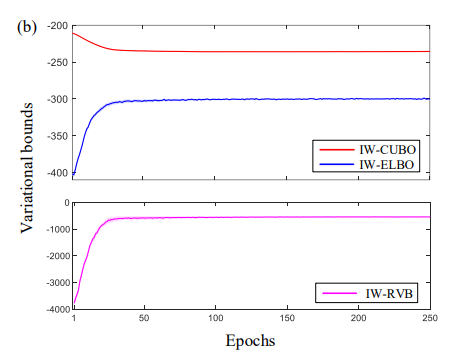
\includegraphics[scale=0.5]{fig1.PNG}
            \caption{f-variational bounds on synthetic data.}
            \label{fig:fig1}
        \end{figure}
    \end{block}
\end{frame}

\begin{frame}{Bayesian neural network}
    \begin{block}{}
        \begin{figure}
            \centering
            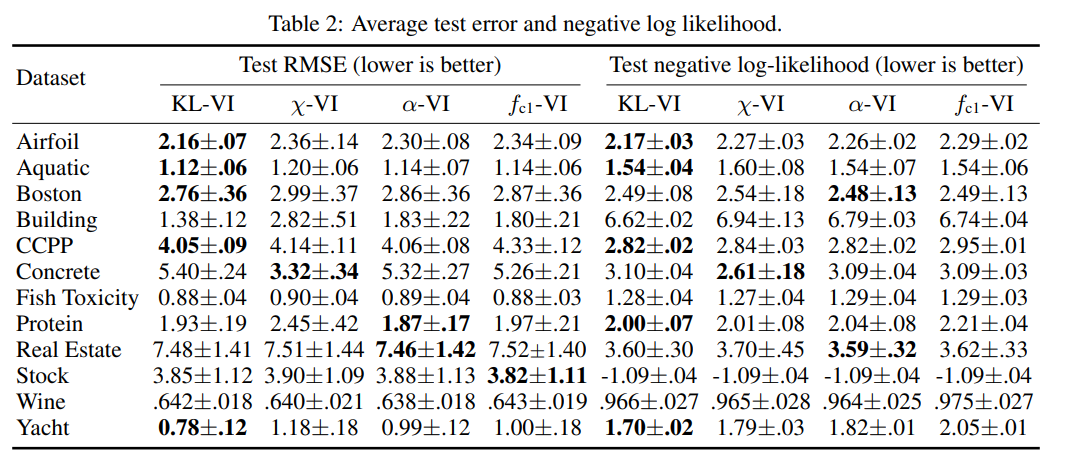
\includegraphics[scale=0.4]{fig2.PNG}
            \caption{BNN test results}
            \label{fig:fig2}
        \end{figure}
    \end{block}
\end{frame}

\begin{frame}{Bayesian variational autoencoder}
    \begin{figure}
        \centering
        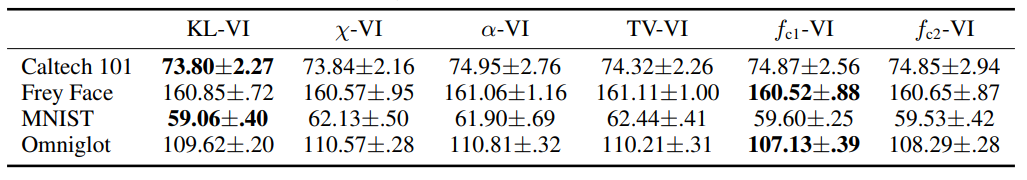
\includegraphics[scale=0.4]{fig3.PNG}
        \caption{Average test reconstruction errors of f-VAEs}
        \label{fig:my_label}
    \end{figure}
\end{frame}
\end{document}
